\documentclass{article}

\usepackage{arxiv}

\usepackage[spanish]{babel}
\usepackage[utf8]{inputenc} % allow utf-8 input
\usepackage[T1]{fontenc}    % use 8-bit T1 fonts
\usepackage{amsmath}       % improved math typesetting
\usepackage{hyperref}       % hyperlinks
\usepackage{cleveref}       % clever references (\cref)
\usepackage{url}            % simple URL typesetting
\usepackage{booktabs}       % professional-quality tables
\usepackage{amsfonts}       % blackboard math symbols
\usepackage{nicefrac}       % compact symbols for 1/2, etc.
\usepackage{microtype}      % microtypography
\usepackage{lipsum}
\usepackage{graphicx}
\usepackage{float}
\usepackage{subcaption}
\crefname{table}{cuadro}{cuadros}
\Crefname{table}{Cuadro}{Cuadros}
\graphicspath{{./images/}{./images/graficos/}}


\title{TP 2.1 - GENERADORES PSEUDOALEATORIOS}


\author{
    Alvaro Tomasino \\
    Ingeniería en Sistemas de Información\\
    Universidad Tecnológica Nacional - FRRO\\
    Zeballos 1341, S2000, Argentina\\
    \texttt{atomasino08@gmail.com} \\
\And
    Melina Aronson \\
    Ingeniería en Sistemas de Información\\
    Universidad Tecnológica Nacional - FRRO\\
    Zeballos 1341, S2000, Argentina\\
    \texttt{melinaaronson@gmail.com} \\
\And
    Tomas Aguilera \\
    Ingeniería en Sistemas de Información\\
    Universidad Tecnológica Nacional - FRRO\\
    Zeballos 1341, S2000, Argentina\\
    \texttt{tomas.aguilera.27@gmail.com} \\
\And
    Juan Bautista Martinelli \\
    Ingeniería en Sistemas de Información\\
    Universidad Tecnológica Nacional - FRRO\\
    Zeballos 1341, S2000, Argentina\\
    \texttt{martinellij4@gmail.com} \\
}




\begin{document}

\maketitle




\begin{abstract}
  El siguiente documento tiene por objetivo introducir uno de los elementos fundamentales para gran parte de las simulaciones, esto son los generadores de números pseudoaleatorios.
\end{abstract}

\keywords{Simulación \and generadores pseudoaleatorios}






\section{Introducción}

\paragraph{Números pseudoaleatorios} Los números pseudoaleatorios se generan de manera secuencial con un algoritmo determinístico, formalmente se definen por:

\begin{itemize}
  \item \textbf{Función de inicialización}: recibe un número (la semilla) y pone al generador en su estado inicial.
  \item \textbf{Función de transición}: transforma el estado del generador.
  \item \textbf{Función de salidas}: transforma el estado para producir un número fijo de bits (0 ó 1).
\end{itemize}

Una sucesión de bits pseudoaleatorios se obtiene definiendo la semilla y llamando repetidamente la función de transición y la función de salidas. Esto implica, entre otras cosas, que una sucesión de números pseudoaleatorios está completamente determinada por la semilla.

Buscamos que una secuencia de números pseudoaleatorios:

\begin{itemize}
  \item No muestre ningún patrón o regularidad aparente desde un punto de vista estadístico,
  \item Dada una semilla inicial, se puedan generar muchos valores antes de repetir el ciclo.
\end{itemize}

\paragraph{Verdaderos números aleatorios} Los números completamente aleatorios (no determinísticos) son fáciles de imaginar conceptualmente, por ejemplo podemos imaginar lanzar una moneda, lanzar un dado una lotería.

En general los números aleatorios se basan en alguna fuente de aleatoriedad física que puede ser teóricamente impredecible (cuántica) o prácticamente impredecible (caótica). Por ejemplo:
\begin{itemize}
  \item random.org genera aleatoriedad a través de ruido atmosférico (el paquete random contiene funciones para obtener números de random.org).
  \item ERNIE, usa ruido térmico en transistores y se utiliza en la lotería de bonos de Reino Unido.
  \item RAND Corporation En 1955 publicó una tabla de un millón de números aleatorios que fue ampliamente utilizada. Los números en la tabla se obtuvieron de una ruleta electrónica.
\end{itemize}

La desventaja de estos métodos es que son costosos, tardados y no reproducibles.

\paragraph{¿Cómo podemos probar la aleatoriedad?} Los tests consisten en tomar muchas secuencias de números aleatorios de un generador dado y someterlas a una serie de pruebas estadísticas. A medida que las secuencias superan más pruebas, aumenta la confianza en la aleatoriedad de los números y, por consiguiente, la confianza en el generador. Sin embargo, dado que esperamos que algunas secuencias parezcan no aleatorias (como por ejemplo obtener diez lanzamientos seguidos de seis en un dado), deberíamos esperar que algunas secuencias fallen al menos en algunas de las pruebas. No obstante, si muchas secuencias fallan las pruebas, deberíamos sospechar.

Una forma de examinar un generador de números aleatorios es crear una visualización de los números que produce. Si bien este tipo de enfoque no debe considerarse un análisis exhaustivo o formal, es una forma rápida y sencilla de obtener una idea general del rendimiento de un generador determinado.

De todas formas resulta conveniente hacer pruebas estadísticas numéricas para evaluar la calidad de los generadores de números pseudoaleatorios.

Hay dos tipos de pruebas:

\begin{itemize}
  \item \textbf{Empíricas}: evalúan estadísticas de sucesiones de números. No demuestran matemáticamente que un generador sea aleatorio; solamente buscan evidencia estadística de comportamiento no aleatorio.
  \item \textbf{Teóricas}: se establecen las características de las sucesiones usando métodos de teoría de números con base en la regla de recurrencia que generó la sucesión. Analizan propiedades matemáticas del generador mismo.
\end{itemize}

En este informe se realizan cuatro tipos de pruebas empíricas: \textbf{Prueba de Frecuencia (Monobit)}, \textbf{Runs Test}, \textbf{Prueba de Bondad de Ajuste $\chi^2$} y \textbf{Prueba de Espera}. También se utilizan tablas e imágenes para mostrar los datos de los distintos generadores y pruebas.



\section{Metodología}
\label{sec:metodologia}

\subsection{Implementación de Generadores de Números Pseudoaleatorios}

\subsubsection{Generador Congruencial Lineal (GCL)}

Es un algoritmo clásico utilizado para producir una secuencia de números pseudoaleatorios. En palabras sencillas, es el mecanismo matemático lógico que muchas computadoras, sistemas y lenguajes de programación usan para simular casos de azar de forma reservada.

Las computadoras, al ser máquinas deterministas (hacen exactamente lo que se les indica), no pueden recrear una situación de azar por su cuenta. Para solucionar esto, el GCL toma un número de partida y muestra de salida un número a simple vista aleatorio, pero que en realidad sigue un patrón fijo.

\paragraph{¿Cómo funciona la matemática en este método?} El GCL calcula el siguiente número de la secuencia aplicando una ecuación lineal simple seguida de una operación de módulo. La fórmula central es:

\begin{equation}
X_{n+1} = (a X_n + c) \bmod m,
\end{equation}

donde:

\begin{itemize}
  \item \textbf{$X_n$ (el valor actual):} Es el número del que partimos en cada ciclo. El primer número de todos ($X_{0}$) se llama \textbf{semilla} (seed). Si corres el algoritmo de nuevo con exactamente la misma semilla y los mismos parámetros, siempre obtendrás la misma secuencia de números.
  \item \textbf{$a$ (el multiplicador):} Una constante por la cual multiplicamos el valor actual.
  \item \textbf{$c$ (el incremento):} Un número fijo que le sumamos al resultado de la multiplicación.
  \item \textbf{$m$ (el módulo):} El límite de nuestra secuencia. La operación $(mod m)$ devuelve el resto de dividir por $m$. Esto actúa como un limitador estricto, asegurando que todos los números generados siempre caigan en el rango entre 0 y $m-1$.
\end{itemize}

Los GCL se introdujeron en 1949 por D.H.Lehemer y son muy populares. La elección de estos parámetros determina la calidad del generador. Queremos un m grande pues el periodo del generador no puede tener más de m elementos.

Y queremos velocidad, en este caso, un valor conveniente para m es el código de palabra (el número máximo de bits que puede procesar el CPU en un ciclo) de la computadora. Los GCL más eficientes tienen m igual a una potencia de 2 (generalmente $2^{32}$ o $2^{64}$) de esta manera la operación módulo se calcula truncando todos los dígitos excepto los últimos 32 ó 64 bits.

\paragraph{El concepto de Período}

Al estar generando número finitos dentro del límite $m$, en algún momento la fórmula va a empezar a generar números repetidos, y a partir de ese momento, la secuencia se va a empezar a repetir en un bucle infinito.

La cantidad de números que el GCL logra generar antes de empezar a repetirse se conoce como período. La idea es seleccionar valores de $a$, $c$ y $m$ tan precisos de manera que el período sea tan gigantesco que su repetición sea prácticamente invisible.

\paragraph{¿Cuál es el período máximo que se puede alcanzar?} Podremos elegir $a$ y $c$ de tal manera que logremos alcanzar el período máximo. Un generador congruencial mixto ($c > 0$) tendrá período completo para todas las semillas si y solo si:

\begin{itemize}
  \item $m$ y $c$ son primos relativos,
  \item $a-1$ es divisible por todos los factores primos de $m$,
  \item $a-1$ es divisible por 4 si $m$ es divisible por 4.
\end{itemize}

Vale aclarar que un periodo grande no determina que el generador congruencial es bueno, debemos verificar que los números que generan se comportan como si fueran aleatorios.

\paragraph{Defectos de los GLCs}

Estos tienden a exhibir defectos, por ejemplo, si se utiliza GCL para elegir puntos en un espacio de dimensión $k$ los puntos van a caer en a lo más $(k! m)^{1/k}$ hiperplanos paralelos k dimensionales, donde $k$ se refiere a la dimensión de $[0,1]^k$.

\paragraph{¿Por qué se eligen?}

Los GCLs continúan siendo utilizados en muchas aplicaciones porque con una elección cuidadosa de los parámetros pueden pasar muchas pruebas de aleatoriedad, son rápidos y requieren poca memoria.

\subsubsection{Método de los cuadrados}

El método de los cuadrados consiste en elevar al cuadrado un número inicial y extraer sus dígitos centrales para usarlos tanto como número pseudoaleatorio como semilla para la siguiente iteración.

Primero se elige la semilla ($X_0$), que consiste en seleccionar un número entero con una cantidad par de dígitos ($n$). Esa semilla se eleva al cuadrado ($X_0^2$), resultando en un número con hasta $2n$ dígitos. Luego se extraen los $n$ dígitos que quedan justo en el medio, y si el resultado tiene menos de $2n$ cifras, se agregan ceros a la izquierda.

Para obtener un número pseudoaleatorio entre 0 y 1 (con distribución uniforme), se divide el número central extraído entre $10^n$. El número central extraído se convierte en la nueva semilla y se repite el proceso.

\subsubsection{Generador de Python}

Se usó el generador de números pseudoaleatorios (PRNG) incorporado en la librería de Python con el módulo \texttt{random}. Este generador usa el algoritmo Mersenne Twister (MT19937), que se destaca por tener un período extremadamente largo de $2^{19937}-1$.

\subsection{Procedimientos de testeo}

\subsubsection{Prueba de bondad de ajuste $\chi^2$ (chi-cuadrado)}

Esta prueba sirve para comprobar si los números generados se comportan como una distribución uniforme entre 0 y 1. La idea es comparar las frecuencias observadas en los datos con las frecuencias esperadas según la distribución teórica.

Se plantean dos hipótesis:

\begin{itemize}
  \item $H_0$: los datos siguen la distribución esperada, es decir, los números están distribuidos uniformemente en $[0,1]$.
  \item $H_1$: los datos no siguen la distribución esperada, es decir, los números no son uniformes.
\end{itemize}

En esta prueba, el intervalo $[0,1]$ se divide en varias partes iguales llamadas celdas. Para la simulación se dividió el intervalo en 10 partes, es decir, se usan 10 celdas. Luego se cuenta cuántos números caen en cada intervalo, y esas cantidades son las frecuencias observadas $O_i$. El valor esperado en cada celda se calcula como:

\begin{equation}
  e_i = n p_i,
\end{equation}

donde $n$ es la cantidad total de números y $p_i$ la probabilidad teórica del intervalo.

Luego se calcula la estadística de prueba como:

\begin{equation}
  \chi^2 = \sum_{i=1}^{c} \frac{(O_i - e_i)^2}{e_i}
  \sim \chi^2_{c-k-1}
\end{equation}

donde $c$ es la cantidad de intervalos y $k$ la cantidad de parámetros estimados a partir de los datos observados.

Se define un nivel de significancia $\alpha$. Este es un valor entre 0 y 1 que indica qué tan "estricto" es el test al rechazar la hipótesis $H_0$. $\alpha$ es la probabilidad de rechazar $H_0$ cuando en realidad $H_0$ es verdadera. El valor crítico, que va a definir la región de rechazo de $H_0$, se calcula como:

\begin{equation}
  \text{valor crítico} = \chi^2_{\mathrm{crit}}(\alpha);
\quad \text{donde} \quad
P\!\left(\chi^2 > \chi^2_{\mathrm{crit}}\right)=\alpha
\end{equation}

En el código este valor se calcula:

\begin{verbatim}
chi_critico = chi2.ppf(1 - alpha, grados_libertad)
\end{verbatim}

Usando $\alpha = 0.05$, es decir, aceptamos un 5\% de riesgo de rechazar $H_0$ cuando en realidad $H_0$ es verdadera.

Si $\chi^2_{\text{calc}} > \chi^2_{\text{crit}}$, entonces se rechaza $H_0$ y los números generados no son suficientemente aleatorios. Caso contrario, los números generados son suficientemente aleatorios para pasar el test.

\subsubsection{Prueba de espera}

Esta prueba se usa para evaluar si una secuencia de números pseudoaleatorios cumple con independencia y uniformidad. La hipótesis nula de la prueba es:

$H_0$: los números son independientes y uniformes.

La idea principal es analizar cuánto se espera entre apariciones sucesivas de números que pertenecen a cierto intervalo del $(0,1)$.

En esta prueba, se elige un subintervalo del $(0,1)$, se calcula su probabilidad, se recorre la secuencia pseudoaleatoria y se anotan las posiciones donde aparecen números que están en el intervalo elegido. Se calculan los tiempos de espera (la cantidad de valores entre dos ocurrencias consecutivas), que siguen una distribución geométrica con parámetro calculado en 2, y se aplica una prueba $\chi^2$ a los tiempos de espera.

\subsubsection{Prueba de Rachas (Runs Test)}

Esta prueba sirve para evaluar si una secuencia de datos ocurre de manera aleatoria o si presenta algún patrón o racha, es decir, una secuencia consecutiva de elementos iguales o del mismo tipo.

La prueba puede detectar demasiadas rachas, es decir, un \textbf{exceso de alternancia} o muy pocas rachas, es decir, un \textbf{agrupamiento o tendencia}.

Se formulan dos hipótesis, al igual que el test anterior, bajo un nivel de significancia $\alpha = 0,05$:

\begin{itemize}
  \item $H_0$: la secuencia es aleatoria.
  \item $H_1$: la secuencia no es aleatoria.
\end{itemize}

Primero, se definen los grupos en los que clasificaremos a los datos. Es común trabajar con secuencias binarias o de dos categorías. Se utilizará el siguiente criterio de agrupamiento:

\begin{itemize}
  \item Si el valor es mayor o igual al promedio de los valores a testear, entonces pertenece al primer grupo, es decir, el valor es de "tipo 1".
  \item Si el valor es menor al promedio, entonces pertenece al segundo grupo, es decir, el valor es de "tipo 2".
\end{itemize}

Así, se cuenta la cantidad de valores de cada tipo:

\begin{itemize}
  \item $n_1$: cantidad de valores del tipo 1,
  \item $n_2$: cantidad de valores del tipo 2.
\end{itemize}

Una racha o run (R) es una secuencia consecutiva de símbolos iguales. Por ejemplo, dado 7 valores, clasificamos a cada si es de tipo 1 o tipo 2. Suponemos que la secuencia de aparición es $2\,1\,2\,1\,1\,1\,2$ siendo "1" si el valor es de tipo 1 y "2" si el valor es de tipo 2. Si separamos:

$2|1|2|111|2$.

Entonces $R = 5$.

Para el análisis de aleatoriedad se calculan:

\begin{itemize}
  \item Esperanza del número de rachas: $E(R) = \frac{2n_1n_2}{n_1+n_2} + 1$.
  \item Varianza:
  $Var(R) = \frac{2n_1n_2\left(2n_1n_2 - n_1 - n_2\right)}
  {(n_1+n_2)^2 (n_1+n_2-1)}$.
\end{itemize}

Con estos datos se transforma a una distribución normal estándar:

\begin{equation}
  Z = \frac{R - E(R)}
  {\sqrt{Var(R)}}
\end{equation}

Finalmente, si $Z > Z_{\alpha/2}$ se rechaza $H_0$, por lo tanto los números generados no son suficientemente aleatorios. Caso contrario, los números generados son suficientemente aleatorios para pasar el test.

Este test tiene ciertas desventajas. Este detecta algunos patrones, no todos, y pierde información al binarizar datos. Tampoco detecta si los valores siguen una distribución uniforme.

\subsubsection{Prueba de frecuencia (Monobit)}

El objetivo de esta prueba es verificar que la proporción de ceros y unos en toda la secuencia sea aproximadamente igual a la esperada en un generador aleatorio real.

Las hipótesis son:

\begin{itemize}
  \item $H_0$: la cantidad de 0 y 1 es equilibrada (la secuencia es aleatoria respecto a esta propiedad), es decir, la probabilidad de 0 y 1 es 0.5.
  \item $H_1$: existe un desbalance significativo entre 0 y 1.
\end{itemize}

En esta prueba, cada bit 0 se convierte al valor $-1$ y cada bit 1 se convierte al valor $+1$, y se suman todos los valores obtenidos:

\begin{equation}
S_n = \sum_{i=1}^{n} x_i.
\end{equation}

El estadístico de prueba es:

\begin{equation}
S_{obs} = \frac{|S_n|}{\sqrt{n}}.
\end{equation}

y el p-valor se calcula como:

\begin{equation}
p = \operatorname{erfc}\left(\frac{S_{obs}}{\sqrt{2}}\right).
\end{equation}

Interpretación: si $p \ge 0.01$, no se rechaza $H_0$ (la secuencia pasa la prueba). Si $p < 0.01$, se rechaza $H_0$ (la secuencia tiene demasiados 0 o demasiados 1).



\section{Resultados}
\label{sec:resultados}

\subsection{Análisis con resultados numéricos}

\paragraph{Resultado para Congruencia Lineal}

\begin{itemize}
  \item Test de Esperas: p-value 0.1228, $\alpha = 0.05$, Pasa: Sí.
  \item Monobit Test: $Z = 2.5298$, $Z_{\text{crítico}} = 1.9600$, Pasa: No.
  \item Runs Test: $Z = -1.3416$, $Z_{\text{crítico}} = 1.9600$, Pasa: Sí.
  \item Test Chi-Cuadrado: $\chi^2 = 20.0000$, $\chi^2_{\text{crítico}} = 16.9190$, Pasa: No.
\end{itemize}

De estos resultados se deduce que, aunque el generador mantiene cierta estructura aleatoria, aparecen sesgos estadísticos. Esto es típico de muchos generadores lineales simples: pueden parecer aleatorios a simple vista, pero pruebas más estrictas revelan patrones internos.

\paragraph{Resultado para Método de los cuadrados}

\begin{itemize}
  \item Test de Esperas: p-value 0.0011, $\alpha = 0.05$, Pasa: No.
  \item Monobit Test: $Z = 3.4000$, $Z_{\text{crítico}} = 1.9600$, Pasa: No.
  \item Runs Test: $Z = 6.2316$, $Z_{\text{crítico}} = 1.9600$, Pasa: No.
  \item Test Chi-Cuadrado: $\chi^2 = 68.0000$, $\chi^2_{\text{crítico}} = 16.9190$, Pasa: No.
\end{itemize}

De estos resultados se deduce que el método degrada rápidamente la calidad de los números generados. Produce ciclos, repeticiones y pérdida de variabilidad, por lo que no es adecuado para aplicaciones reales.

\paragraph{Resultado para \texttt{random()} de Python}

\begin{itemize}
  \item Test de Esperas: p-value 0.0871, $\alpha = 0.05$, Pasa: Sí.
  \item Monobit Test: $Z = 0.7589$, $Z_{\text{crítico}} = 1.9600$, Pasa: Sí.
  \item Runs Test: $Z = -0.9492$, $Z_{\text{crítico}} = 1.9600$, Pasa: Sí.
  \item Test Chi-Cuadrado: $\chi^2 = 11.6800$, $\chi^2_{\text{crítico}} = 16.9190$, Pasa: Sí.
\end{itemize}

De estos resultados se deduce que este generador produce números con comportamiento cercano al aleatorio ideal para este conjunto de pruebas. Es el más confiable de los tres para simulaciones y aplicaciones generales.

\subsection{Análisis visual con bitmap}

Se generaron 40.000 números para armar una cuadrícula de $200 \times 200$ píxeles.

\paragraph{GCL con parámetros buenos} Usando $a = 1.664.525$, $c = 1.013.904.223$ y $m = 2^{32}$, el generador produjo un mapa de bits con ruido uniforme, sin patrones geométricos visibles.

\paragraph{GCL con parámetros malos} Usando $a = 106$, $c = 1283$ y $m = 6075$, se observan patrones de franjas y líneas diagonales, demostrando baja calidad.

\begin{figure}[H]
    \centering

    \begin{subfigure}{0.48\textwidth}
        \centering
        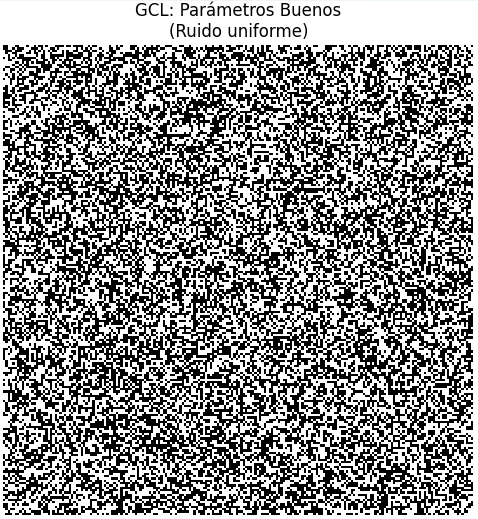
\includegraphics[width=\linewidth]{imagen1a.png}
        \caption{Parámetros buenos}
        \label{fig:imagen-1a}
    \end{subfigure}
    \begin{subfigure}{0.48\textwidth}
        \centering
        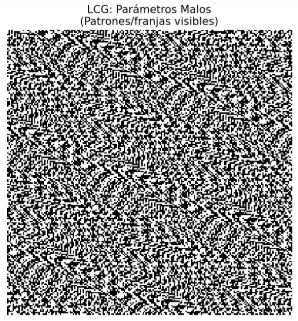
\includegraphics[width=\linewidth]{imagen1b.png}
        \caption{Parámetros malos}
        \label{fig:imagen-1b}
    \end{subfigure}

    \caption{GCL}
    \label{fig:gcl}
\end{figure}

\paragraph{Método de los cuadrados} Muestra una degradación hacia el color negro (valor 0), confirmando la tendencia del algoritmo a converger a 0 cuando los dígitos centrales de la semilla se anulan.

\paragraph{Generador de Python} Muestra ruido uniforme sin patrones geométricos ni tendencias de agrupamiento.

\begin{figure}[H]
    \centering

    \begin{subfigure}{0.3\textwidth}
        \centering
        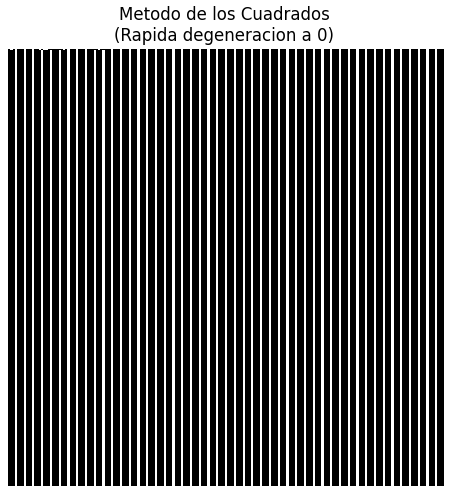
\includegraphics[width=\linewidth]{imagen2a.png}
        \caption{Método de los cuadrados}
        \label{fig:imagen-2a}
    \end{subfigure}
    \begin{subfigure}{0.3\textwidth}
        \centering
        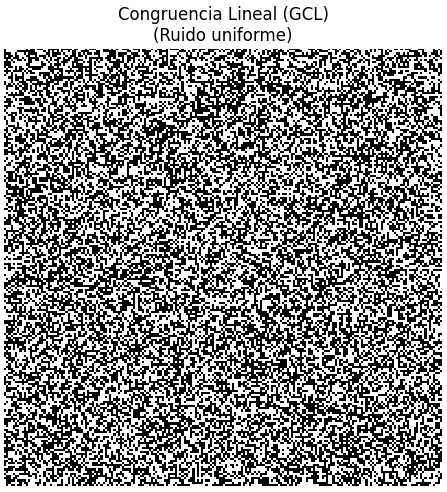
\includegraphics[width=\linewidth]{imagen2b.png}
        \caption{GCL}
        \label{fig:imagen-2b}
    \end{subfigure}
    \begin{subfigure}{0.3\textwidth}
        \centering
        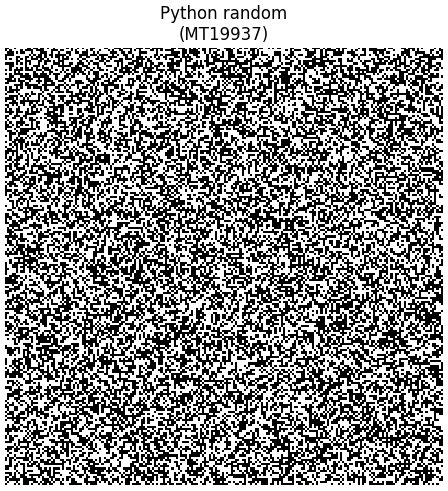
\includegraphics[width=\linewidth]{imagen2c.png}
        \caption{Python}
        \label{fig:imagen-2c}
    \end{subfigure}

    \caption{Comparación de generadores}
    \label{fig:generadores}
\end{figure}


\subsection{Comparación de tests}

\begin{table}[H]
  \centering
  \begin{tabular}{lccccc}
    \toprule
    Generador & Tipo de generador & Test 1: Esperas & Test 2: Monobit & Test 3: Runs Test & Test 4: Chi-Cuadrado \\
    \midrule
    GLC & Pseudoaleatorio & OK & ERROR & OK & ERROR \\
    Cuadrados  & Pseudoaleatorio & ERROR & ERROR & ERROR & ERROR \\
    Python     & Pseudoaleatorio & OK & OK & OK & OK \\
    \bottomrule
  \end{tabular}
  \caption{Comparación de tests}
  \label{tab:comparacion-tests}
\end{table}

\subsection{Comparación de generadores}

El método de los cuadrados es el menos eficiente. A medida que avanza la generación de números, se degrada rápidamente hacia el valor 0, perdiendo su aleatoriedad.

El GCL mostró buenos resultados, pero depende de los parámetros que se elijan. Con parámetros adecuados, mantiene la estabilidad, pero si los parámetros son inadecuados aparecen patrones visibles y repeticiones que afectan la calidad de los números generados.

El generador de Python (MT19937) es el más estable, manteniendo un ruido uniforme constante gracias a su período extenso de $2^{19937}-1$.



\section{Discusión}

Observando los gráficos, se puede ver que, tomando el primer par de resultados, uno presenta un ruido uniforme, simulando casos de secuencias verdaderamente aleatorias, y el otro, con otra selección de parámetros, presenta un patrón claramente visible, por lo que no es una simulación válida.

En el segundo trío de imágenes, lo que cambia no son los parámetros, sino los generadores utilizados. En el primero, usamos el método de los cuadrados, que presenta un patrón visible (por el color negro predominante), mientras que el generador de congruencia lineal y el de Python (MT19937) logran un ruido uniforme, comportándose de forma más cercana a las secuencias aleatorias ideales.




\section{Conclusiones}

Los números pseudoaleatorios son herramientas fundamentales en áreas como la informática, la estadística y la simulación. Aunque están bajo algoritmos definidos, si se usan los parámetros y los valores adecuados podemos simular casos de secuencias verdaderamente aleatorias y el comportamiento de sistemas sin experimentar directamente sobre ellos, siendo una opción de obtener conclusiones con mucho menos costos.

En definitiva, los números pseudoaleatorios permiten resolver problemas complejos mediante modelos computacionales eficientes, pero su correcta utilización depende de comprender sus limitaciones y validar adecuadamente la calidad de las secuencias producidas.




\nocite{*}

\bibliographystyle{unsrturl}
\bibliography{references}

\end{document}


